\section{System Considerations}
If not explicitly mentioned, the system's settings are as follows:
\subsubsection*{Ensemble}
$N$ particles in a box of volume $V$ and temperature $T$ are considered.
The closed box is placed in an external heat bath, hence the total energy is not fixed and the probability $P_i$ for a given State $\ket{i}$ with Energy $E_i$ and $\beta \mathrel{\mathop:}= \frac{1}{kT}$ is given by
\begin{align}
	P_i = \frac{1}{Z}\exp\left(-\beta E_i\right)\text{, and }
	Z = \sum_k \exp\left(-\beta E_k\right).
\end{align}
Such an ensemble is called canonical or NVT.

\subsubsection*{Potential and Energy}
The particles are interacting via a normed Lennard-Jones Potential
\begin{align}
\label{LJPot}
	V_{ij} = 4\left(\frac{1}{r_{ij}^{12}} - \frac{1}{r_{ij}^6} + \frac{2^7 - 1}{2^{14}}\right),
\end{align}
such that $V_{ij}=0$, if $r_{ij} = 2\sqrt[6]2$.
The total energy $E_n$ of the system in a state $\ket{n}$ is given by the expression
\begin{align}
	E_n = \sum_i\sum_{j\neq i}V_{ij}.
\end{align}
\newpage
\subsubsection*{Periodic Boundary Conditions}
For both implementations, periodic boundary conditions (PBC) will be used.
With PBC there are two important consequences for our System. \\
First, when a particle reaches the border of the System, it is not reflected back, but transfered to the other side of the box.
\begin{figure}[h!]
\centering
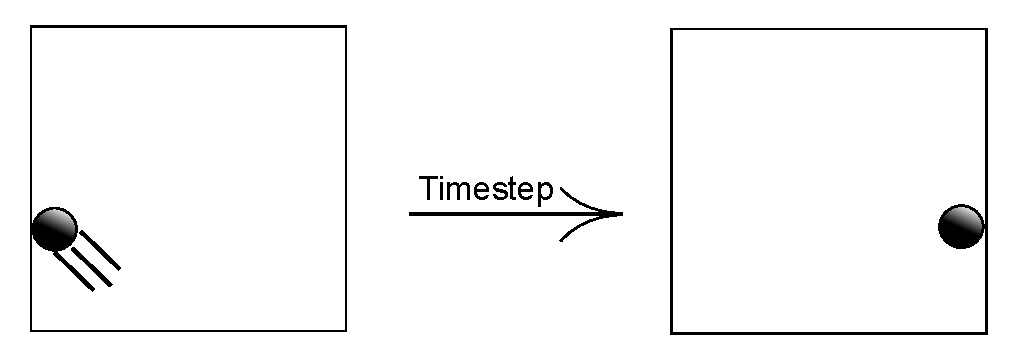
\includegraphics[width=0.8\textwidth]{PBCjump.pdf}
\caption[PBC: Jump Case]{A particle in a box with PBC jumps from one side to the other.}
\end{figure}
Second, particles can interact with images of other particles behind the border of the box. As a result, the distance vector between two particles is not definite. 
\begin{figure}[h!]
\centering
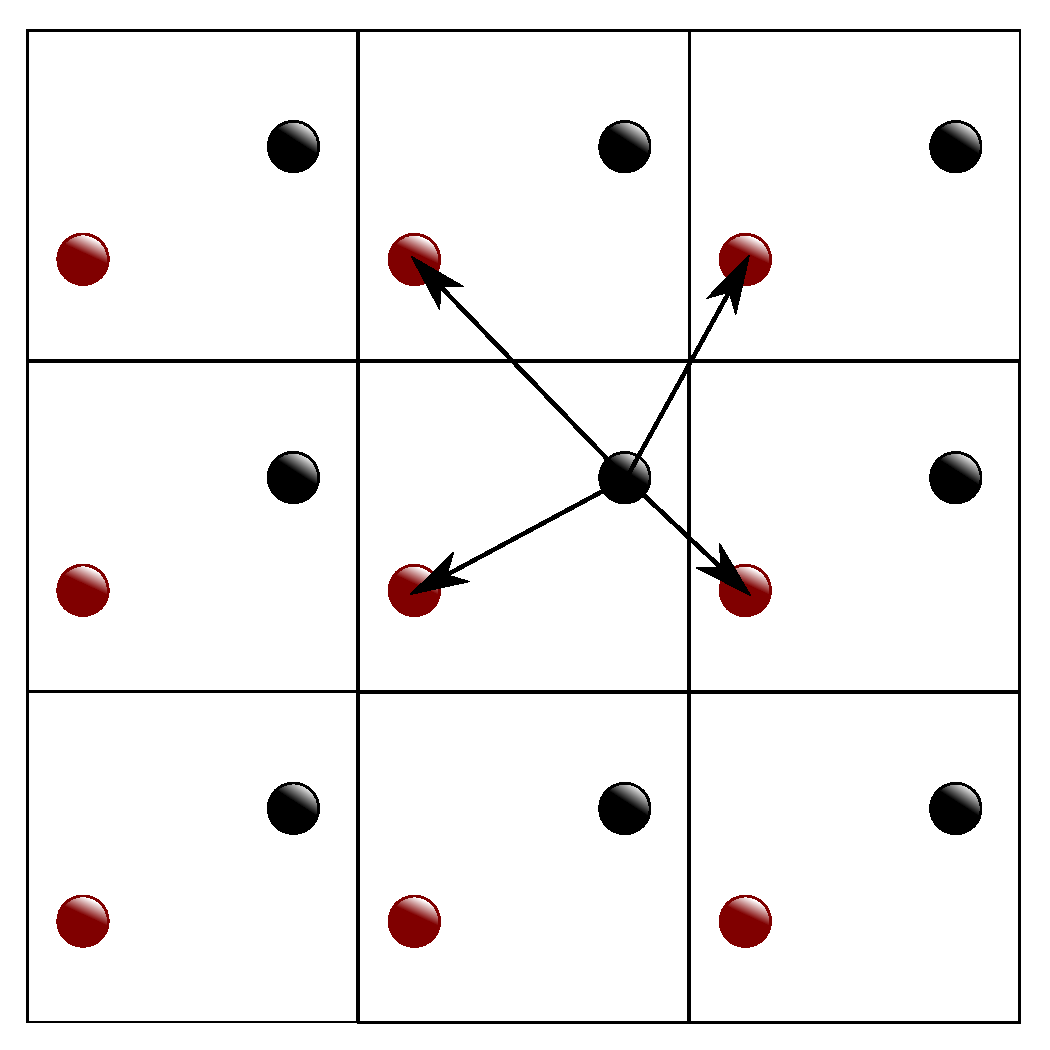
\includegraphics[width=0.8\textwidth]{PBCinteraction.pdf}
\caption[PBC: Interaction Case]{In the middle is the main simulation box with two particles being simulated, the surounding eight boxes are periodic images of the main box. The distance between the two particles is not definite with PBC because there are multiple ways to get from one particle to the other.}
\label{PBCinteraction}
\end{figure}
Of course a particle doesn't interact with all the images of one and the same particle, thats why the minimum image convention is used, which means a particle only interacts with the closest image of another particle. In figure (\ref{PBCinteraction}) that would be the image to the right middle.





